\section{Auxiliary circle and the affine map}

Let $\ell$ be the major axis and let $O$ be the center of the ellipse. Recall that the ellipse has semi-major axis $a$ and semi-minor axis $b$. Consider the \emph{major-axis circle} $\mathcal C$: the circle centered at $O$ with radius $a$ (so its diameter equals the major axis length $2a$). This is also the standard \emph{auxiliary circle} associated to the ellipse.

Define the affine map $\Phi$ geometrically as follows. For any point $P$ in the plane, let $P_T$ be the foot of the perpendicular from $P$ to $\ell$. On the same perpendicular line $P_TP$ choose a point $P_0$ on the same side of $\ell$ as $P$ such that
\begin{equation}
  P_TP_0=\frac{b}{a}\,P_TP.
\end{equation}
Then set $\Phi(P):=P_0$.

Equivalently, $\Phi$ fixes $\ell$ pointwise and scales all lengths perpendicular to $\ell$ by the constant factor $b/a$. This map sends lines to lines, preserves parallelism, and scales all areas by $b/a$. In the standard auxiliary circle construction, $\Phi$ maps $\mathcal C$ to the ellipse.

\paragraph{Tangents via secants (Newton's 1687 viewpoint).}
Newton often treats a tangent as the \emph{ultimate position} of a secant: if $A$ is a point on the curve and $B$ is a nearby point, then the chord line $AB$ approaches the tangent line at $A$ as $B\to A$ (in Newton's 1687 language, as one takes the ``ultimate ratio''). In our setting this provides an alternative justification for the fact that $\Phi$ carries circle tangents to ellipse tangents.

Indeed, let $A_0\in\mathcal C$ correspond to $A=\Phi(A_0)$ on the ellipse, and let $B_0\in\mathcal C$ correspond to $B=\Phi(B_0)$. Since $\Phi$ is affine, it maps the secant (chord) line $A_0B_0$ to the secant line $AB$, and it preserves incidences and parallelism. As $B_0\to A_0$, the secant line $A_0B_0$ approaches the tangent to $\mathcal C$ at $A_0$, while $AB$ approaches the tangent to the ellipse at $A$. Therefore, in the same limiting (secant-to-tangent) sense, $\Phi$ maps the circle tangent at $A_0$ to the ellipse tangent at $A$.

\begin{figure}[t]
  \centering
  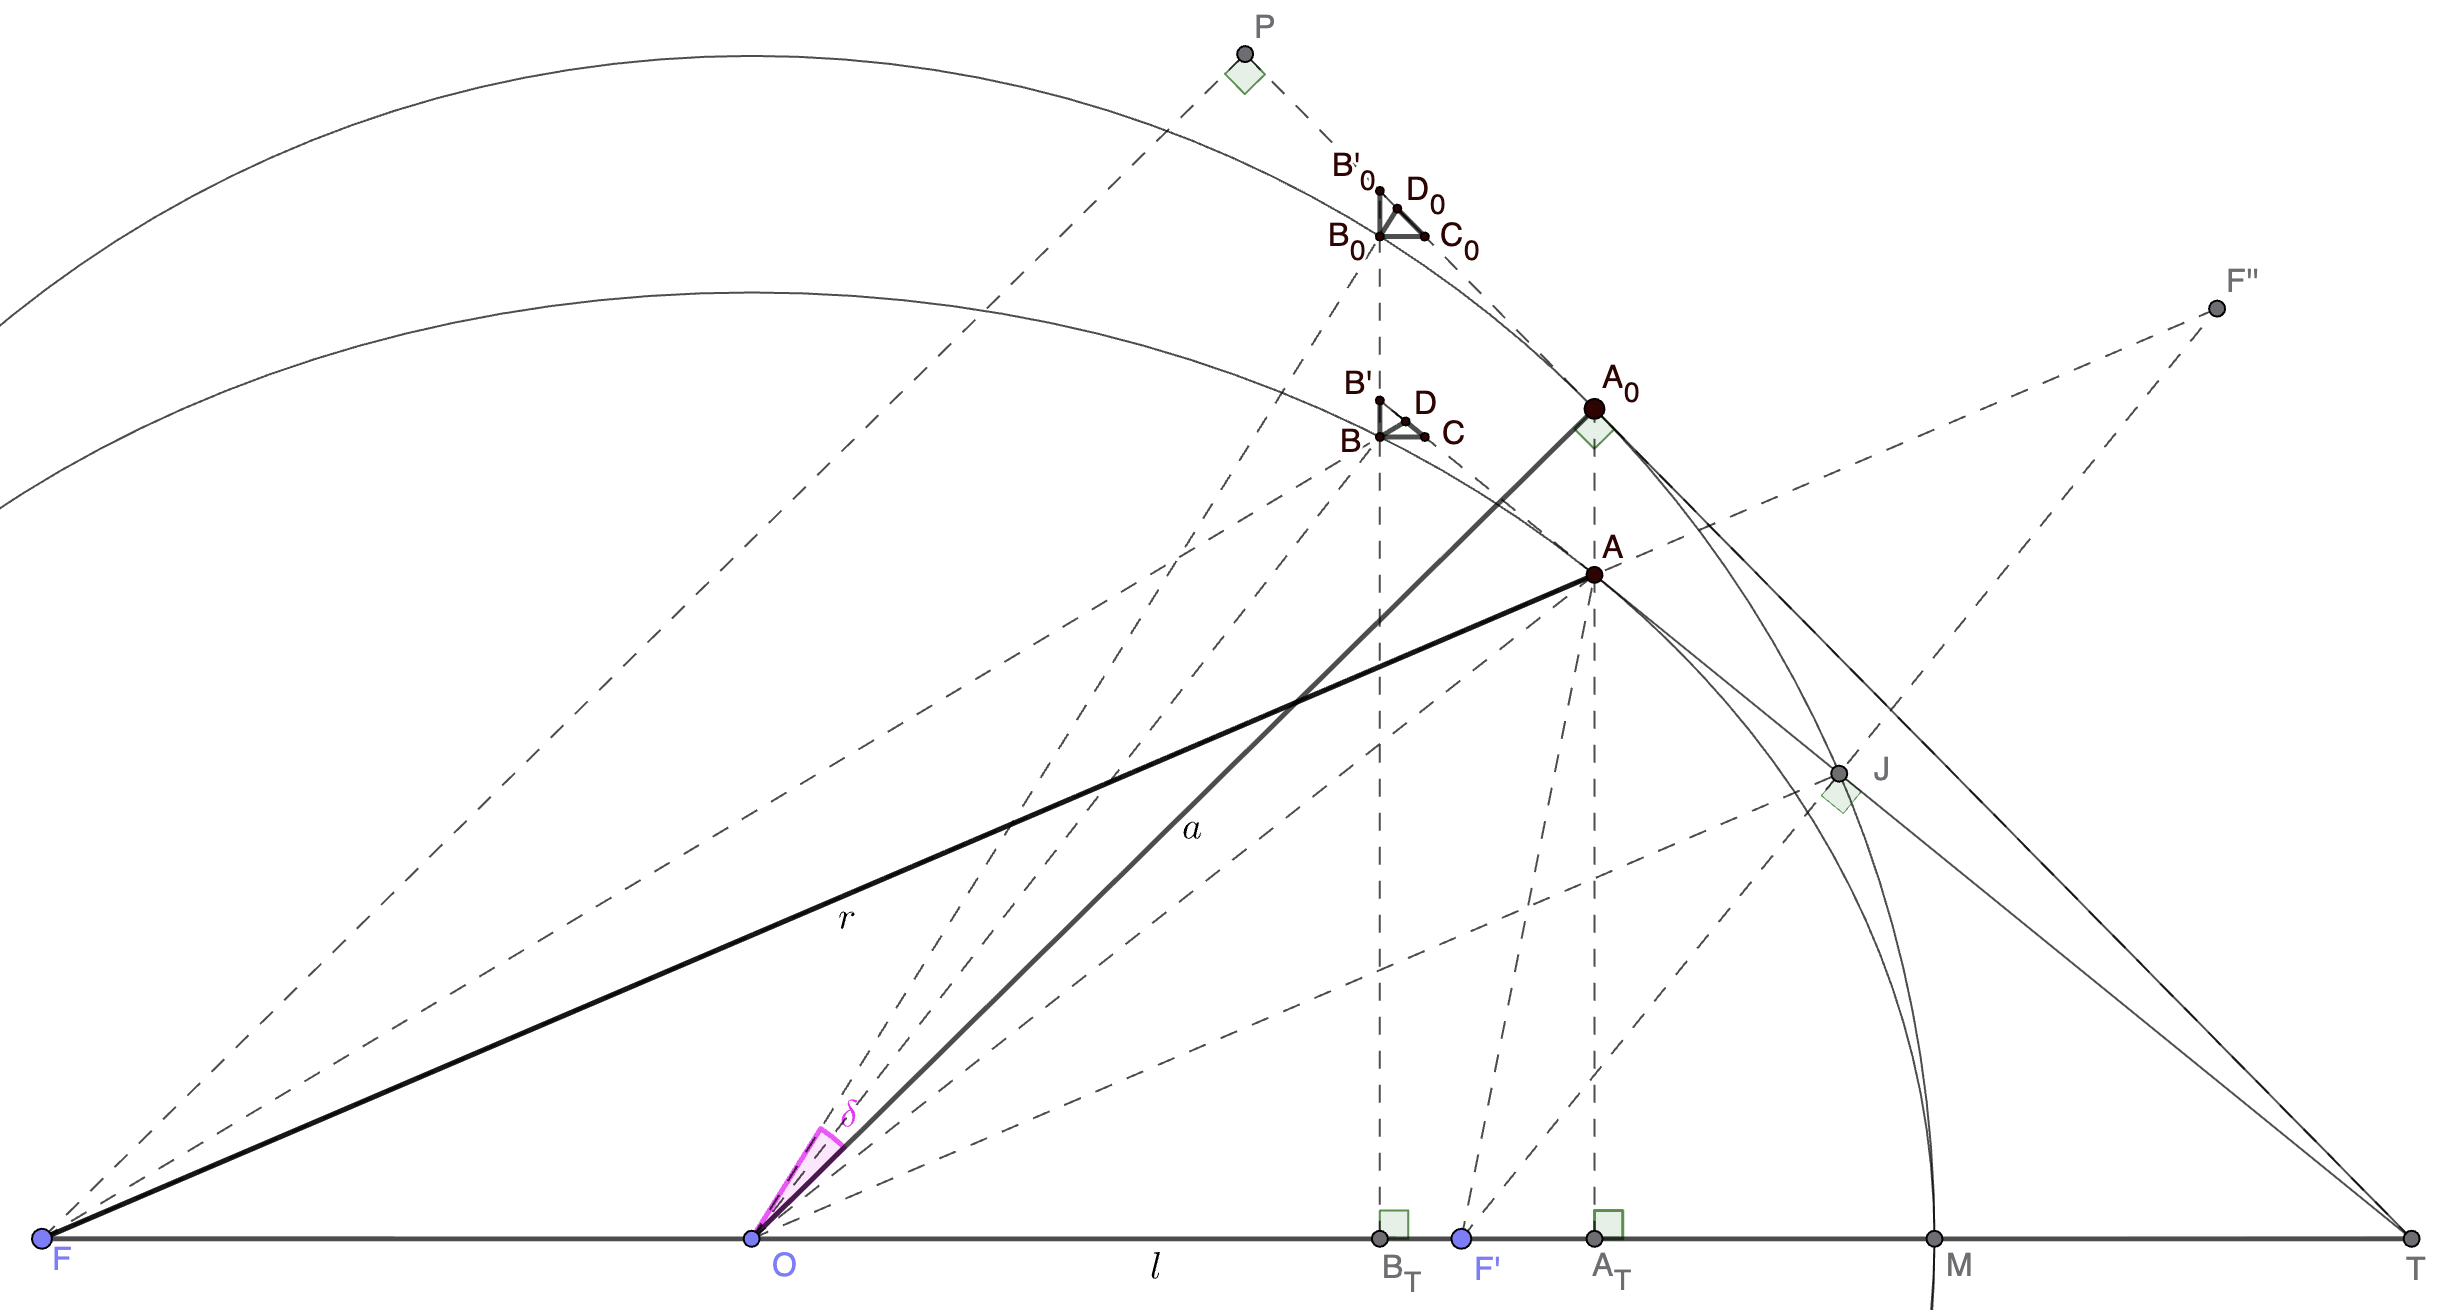
\includegraphics[width=\linewidth]{assets/images/MotionFigure.png}
  \caption{Affine relation of motion between the auxiliary circle and the ellipse.}
  \label{fig:affine-relation-of-motion}
\end{figure}

A few simple geometric consequences we use repeatedly:
\begin{itemize}
  \item Straight lines map to straight lines under $\Phi$.
  \item Horizontal lengths (parallel to $\ell$) are unchanged by $\Phi$.
  \item Vertical lengths (perpendicular to $\ell$) scale by $b/a$.
  \item Parallel lines stay parallel under $\Phi$, and ratios of lengths along such lines are unchanged by $\Phi$.
  \item Areas scale by $b/a$.
  \item The inverse map $\Phi^{-1}$ sends $\Phi(A)$ back to $A$ and scales vertical lengths by $a/b$.
\end{itemize}
Even though Newton (1687) did not describe affine transformations explicitly, he was well aware of these properties and applied them throughout his books. He also used clever polygonal approximations to treat areas under curves (a method far ahead of its time).
